\section{Prepogibanje kvadrata}
\label{pogl:prepog_kvadrata}

Vzemimo v roke kvadraten list papirja in poglejmo, kaj lahko z njegovim prepogibanjem dobimo. V tem poglavju se bomo ukvarjali s preprostimi konstrukcijami, kot so konstrukcija enakostraničnega trikotnika, razdalje $\sqrt{k}$ za poljuben $k \in \mathcal{O}$, razdelitve daljice na enako število delov; pogledali si bomo vse tri Hagove izreke o razmerjih, na katere specifični pregibi kvadratnega lista papirja razdelijo njegove stranice; na koncu pa si bomo končno pogledali še konstrukcije rešitev dveh starogrških problemov, zaradi katerih smo se sploh začeli ukvarjati s temo origamija.

\subsection{Nekaj kratkih in zanimivih konstrukcij za uvod}

% kot 60° (smo že pri algebri)
% enakostranični trikotnik (smo že pri algebri, ma lahko še enkrat, pa več načinov)
% kvadratni koren od 2, od k

\subsubsection*{Konstrukcija števila $\sqrt{r}$}

Vzemimo $r \in \Q^+$ in si poglejmo naslednjo konstrukcijo (vzeto iz~\cite[str.\ 58]{hull2013}):
Imejmo točko $A (0, 1) $ in premico $y = -1$. Na ordinatni osi označimo točko $B (0, -\frac{r}{4})$ in naredimo pregib skoznjo, ki točko $A$ položi na premico $y = -1$. Njena zrcalna slika je $A' (t, 0) $ za nek $t \in \R$ (slika~\ref{fig:konstrukcija_korena}).

\begin{figure}[h]
    \centering
    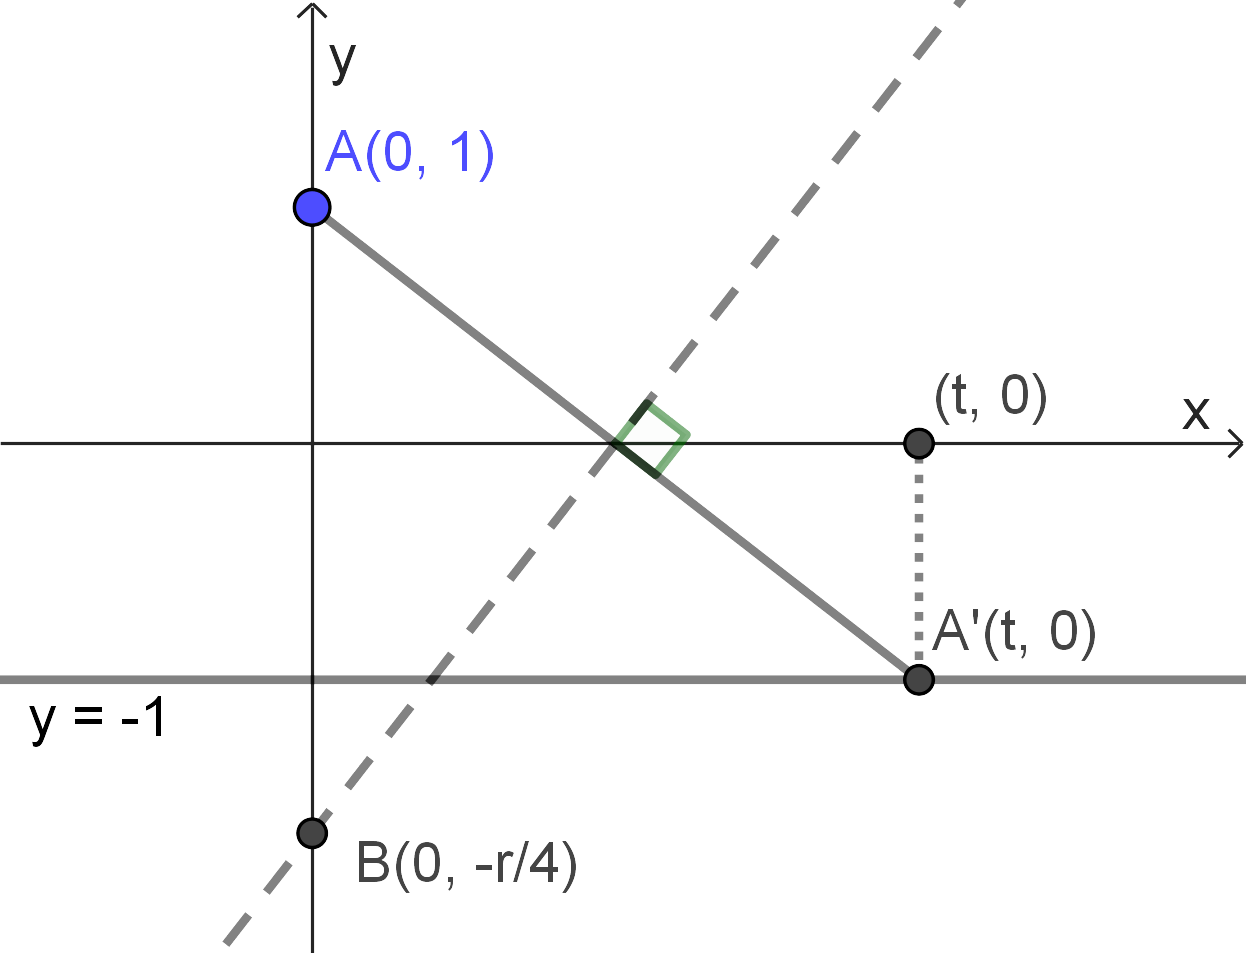
\includegraphics[width=0.5\textwidth]{images/kvadratni_koren.png}
    \caption[Konstrukcija korena]{Konstrukcija števila $\sqrt{r}$ za poljuben $r \in \Q^{+}$.}
    \label{fig:konstrukcija_korena}
\end{figure}

Pregib poteka skozi točko $B$ in razpolovišče daljice $AA'$, torej je njegov koeficient $k_B = \frac{r}{2t}$ (izpeljavo prepuščamo bralcu). Ker je pregib simetrala daljice $AA'$, njena nosilka pa ima koeficient $k_A = - \frac{2}{t}$, dobimo
\begin{align*}
    k_B &= - \frac{1}{k_A},\\
    \frac{r}{2t} &= \frac{t}{2},\\
    r &= t^2 \text{ oz. } t = \sqrt{r}.
\end{align*}
Na koncu le še prepognemo pravokotnico na abscisno os skozi točko $A'$ in tako dobimo točko $(\sqrt{r}, 0)$. Torej smo konstruirali število $\sqrt{r}$ za poljuben $r \in \Q^{+}$.



\subsection{Razdelitev daljice na $n$ enakih delov}

Stranico kvadrata želimo razdeliti na $n$ enakih delov, kjer je $n \in \N$ poljuben. Za $n = 2^t, t \in \N_0$ je to čisto enostavno, saj samo prepolavljamo razdalje med pregibi, dokler ne dosežemo cilja. Če je $n$ sod, vendar ni potenca $2$, torej $n = 2^t(2m + 1)$, kjer sta $t, m \in \N$, stranico najprej razdelimo na $2^t$ delov, nato pa moramo vsakega izmed njih razdeliti na $2m + 1$ (liho število) delov. Izziv tega problema je torej v razdelitvi daljice na liho število delov. Ko bomo zo zmogli, jo bomo znali razdeliti na $n$ delov za vsak $n \in \N$.

V dokazu izreka~\ref{izr:podpolje} smo za poljuben $a \in \R$ znali konstruirati razdaljo $1/a$, kar bi lahko uporabili za razdelitev neke daljice na $a$ enakih delov -- konstruirano razdaljo $1/a$ bi $a$-krat prenesli naprej. Načinov reševanja tega problema pa se je skozi zadnja desetletja oblikovalo še veliko več; tu si bomo pogledali še \textcolor{red}{koliko?} metode.

\subsubsection*{Metoda križajočih se diagonal}

Metoda nima uradnega prevoda niti uradnega imena, jo pa tako imenuje Robert J.\ Lang v svojem članku~\cite{lang1988}. Njena konstrukcija je prikazana na sliki \textcolor{red}{referenca na sliko, ustvari sliko al pej kopirej hull2020 str.\ 14 al pej hull2018 str.\ 38}. Najprej kvadrat dvakrat prepognimo na pol -- enkrat po diagonali skozi oglišči $A$ in $C$ in drugič po vertikali. Nato prepognemo po diagonali (skozi oglišče $B$) še desni pokončen pravokotnik. Presečišče obeh diagonal označimo s točko $P$ in naredimo skoznjo prepogib, ki je pravokoten na horizontalno stranico kvadrata.

\begin{trditev}
    \label{trd:kriz_diag_3}
    Zadnji pregib iz zgornjega opisa konstrukcije razdeli horizontalno stranico kvadrata v razmerju $2:1$.
\end{trditev}

\begin{dokaz}
    Dokazujemo lahko na več načinov:
    \begin{enumerate}
        \item \textit{Analitičen pristop:} Kvadrat postavimo v evklidsko ravnino tako, da je spodnje levo oglišče kvadrata v koordinatnem izhodišču in spodnje desno v točki $(1, 0)$. Obe diagonali izrazimo z enačbama premic. Glavna diagonala ima enačbo $y = x$, diagonala pravokotnika pa $y = -2x + 2$. Točka $P$ je njuno presečišče in ima tako koordinati $(2/3, 2/3)$.
        \item \textit{Preko podobnih trikotnikov:} Z opisanimi prepogibi v tem kvadratu konstruiramo več trikotnikov. Njihova oglišča označimo tako, kot kaže slika \textcolor{red}{naredi in referiraj sliko, str. 38 v hull2013; ampak predrugači imena oglišč (glej nadaljevanje tega dokaza)}. Iz podobnosti trikotnikov $\triangle AGP$ in $\triangle ABC$ sledi, da je trikotnik $\triangle AGP$ enakokrak. Naj bo dolžina njegovih krakov $x$. Potem je $|AG| = |GP| = x$ in $|GB| = 1 - x$. Iz podobnosti trikotnikov $\triangle EFB$ in $\triangle PGB$ sledi
        \begin{align*}
            \frac{|EF|}{|FB|} &= \frac{|PG|}{|GB|}, \\
            \frac{1}{\frac{1}{2}} &= \frac{x}{1 - x}, \\
            x &= \frac{2}{3}.
        \end{align*}
    \end{enumerate}
\end{dokaz}

Po konstrukciji pregiba, ki zgornjo stranico kvadrata razdeli v razmerju $2:1$, desni pravokotnik (s stranico $DE$) po vertikali prepognemo še na pol. S tem smo stranico kvadrata razdelili na tri enake dele.

Razdelitev stranice kvadrata na štiri dele je očitna -- kvadrat v vertikalni smeri dvakrat prepognemo na pol.

Stranico razdelimo na pet delov na podoben način kot na tri. Naredimo enak pregib po glavni diagonali, nato pa zgornjo stranico razdelimo v razmerju $3:1$ (to znamo storiti). S tem smo na desni strani kvadrata dobili pokončen pravokotnik s horizontalno stranico, dolgo četrt stranice kvadrata. Naslednji pregib je, kot prej, diagonala tega pravokotnika (tista skozi oglišče $B$). Presečišče te in glavne diagonale je točka, ki je od desne stranice oddaljena za $1/5$ (dokaz je analogen tistemu za trditev~\ref{trd:kriz_diag_3}). Naredimo vertikalen pregib skozi točko $P$ in s tem zgornjo stranico kvadrata razdelimo v razmerju $4:1$. Na koncu še levi del te stranice razdelimo na štiri dele. S tem smo celotno stranico razdelili na pet skladnih delov.

Zgornji postopek lahko posplošimo na poljuben $n \in \N$. Kot smo videli v konkretnih primerih za $n = 3, 4$ in $5$, smo si pomagali z vnajprejšnjo razdelitvijo stranice na $n-1$ število enakih delov (kar smo zmogli storiti). Dokaz naslednje trditve bo tako temeljil na indukciji.

\begin{trditev}[Metoda križajočih se diagonal za splošen $n$]
    Naj bo $n \in \N, n > 2$. Kvadrat $ABCD$ s stranico dolžine $1$ prepognemo po diagonali $AC$, potem pa stranico $DC$ s točko $E$ razdelimo v razmerju $(n-2):1$. Naredimo pregib novonastalega pravokotnika skozi točki $B$ in $E$. Presečišče te in glavne diagonale je točka $P$, ki je od desne stranice kvadrata oddaljena za $1/n$.
\end{trditev}

\begin{dokaz}
    Za $n = 1$ in $n = 2$ ni kaj dokazovati -- v prvem primeru pregiba sploh ni, v drugem primeru stranico prepolovimo.

    \textit{Baza indukcije:} Vemo že, da trditev drži za $n = 3, 4, 5$.

    \textit{Indukcijska predpostavka:} Predpostavimo, da znamo stranico razdeliti na $n$ enakih delov.

    \textit{Indukcijski korak:} Dokazujemo, da znamo stranico razdeliti na $n+1$ enakih delov. Po navodilih za konstrukcijo najprej stranico $DC$ s točko $E$ razdelimo v razmerju $(n-1):1$ (kot če bi jo razdelili na $n$ skladnih delov, ampak označimo le zadnji prpogib). To po indukcijski predpostavki znamo storiti. S prepogibom skozi oglišče $B$ in točko $E$ dobimo, kot presečišči obeh diagonal, točko $P$. Potem pa podobno kot pri dokazu trditve~\ref{trd:kriz_diag_3} dokažimo, da leži točka $P$ na želeni razdalji od desne stranice kvadrata:
    \begin{enumerate}
        \item \textit{Analitičen pristop:} Naj bo oglišče $A$ koordinatno izhodišče in oglišče $B$ točka $(1, 0)$. Premica, ki je nosilka diagonale $AC$, ima tako enačbo $y = x$, nosilka diagonale $CE$ pa $y = -nx + n$. Točka $P$ je njuno presečišče in ima tako koordinate $(n/(n+1), n/(n+1))$. Torej je od desne stranice kvadrata res oddaljena za $1/(n+1)$.
        \item \textit{Preko podobnih trikotnikov:} Označimo oglišča trikotnikov, kot kaže slika \textcolor{red}{SLIKA plus REFERENCA}. Trikotnik $\triangle AGP$ je enakokrak in njegova kraka označimo z $x$. Iz razmerij dolžin stranic podobnih trikotnikov $\triangle EFB$ in $\triangle PGB$ sledi
        $$ \frac{|EF|}{|FB|} = \frac{|PG|}{|GB|} \Rightarrow \frac{1}{\frac{1}{n}} = \frac{x}{1 - x} \Rightarrow n - nx = x \Rightarrow x = \frac{n}{n+1}. $$
        Točka $P$ je od desne stranice kvadrata res oddaljena za $x - 1 = 1/(n + 1)$.
    \end{enumerate}

\end{dokaz}

\begin{posledica}
    Poljubno daljico znamo razdeliti na $n$ skladnih delov za vsak $n \in \N$.
\end{posledica}

\begin{dokaz}
    Vzemimo neko daljico poljubne dolžine. Ker znamo konstruirati pravokotnice skozi točke in prenašati razdalje, lahko konstruiramo kvadrat, katereda zgornja stranica dana daljica \textcolor{red}{(spet kakšna slikca več korakov)}. Po zgornji trditvi jo znamo razdeliti v razmerju $(n-1) : 1$ za vsak $n \in \N$. Potem moramo njen daljši del razdeliti na $n-1$ skladnih delov. To storimo na enak način kot prej -- konstruiramo manjši kvadrat s to novo stranico in ponovimo postopek. Ustavimo se, ko na nekem koraku stranico kvadrata razdelimo v ramerju $1:1$. Takrat bo zgornja stranica oz. dana daljica razdeljena na $n$ skladnih delov.
\end{dokaz}

\subsubsection*{Metoda2}

\subsubsection*{Metoda3}

\subsubsection*{Metoda4}

\textcolor{red}{Več metod (vsaj tri?), na koncu daš Hagovo metodo in iz tega začneš z novim podpoglavjem -- Hagovi izreki. Matode pred tem: Hull2013 (str.\ 36--40)}


\subsection{Hagovi izreki}

S prepogibanjem kvadratnega lista papirja se je veliko ukvarjal Kazuo Haga, sicer japonski profesor biologije. V svojem delu \emph{Origamics: Mathematical Explorations Through Paper Folding}~\cite{haga2008} je tako med drugim formuliral tri izreke, ki jih poznamo pod imenom \emph{Hagovi izreki}.



\textcolor{red}{Konstrukcija poljubnega $a/b \in \Q$~\cite[str.\ 20--21]{lang2013}}

\textcolor{red}{Hull2013, activity 11 (str. 103--)}

\subsubsection{Prvi Hagov izrek}

\textcolor{red}{PLUS poslošitev.}

\subsubsection{Drugi Hagov izrek}

\textcolor{red}{PLUS poslošitev.}

\subsubsection{Tretji Hagov izrek}

\textcolor{red}{PLUS poslošitev.}





\subsection{Reševanje nerešljivih starogrških problemov}
\label{podpogl:starogrskiproblemi}

% - trisekcija kota (Abe, Justin)
% - podvojitev kocke (Messer, Beloch)

% Naštej vse tri. Onega od $\pi$ se ne da rešiti?
% reševanje dveh starogrških problemov, ki ju z evklidskimi orodji -- dokazano -- ne znamo rešiti; to sta \emph{podvojitev kocke} (oz. konstrukcija $\sqrt[3]{2}$) in \emph{trisekcija kota}. Izkaže se, da se da vsakega od njiju rešiti celo na več kot en način! (to je omenjeno v 2.3, tko da trisekcija mora imet več načinov, čene popravi)


\subsubsection{Trisekcija kota}
\label{podpogl:trisekcija}

\textcolor{red}{Motivacija za ta problem?}

Kot $90^\circ$ znamo tretjiniti z neoznačenim ravnilom in šestilom, saj znamo konstruirati kot $30^\circ$. Težava je, da ne obstaja konstrukcija, s katero na tri skladne kote razdelimo \emph{poljuben} kot. V~\cite[str.\ 77--78]{jerman1998} je dokaz o nezmožnosti trisekcije kota $60^\circ$. Avtor se pri tem sklicuje na izrek~\ref{izr:evkl_konstr} in opombo~\ref{op:razseznost_obsega_evkl} in podpoglavja~\ref{podpogl:evkl_konstruktibilnost}.

% SPODNJI DOKAZ JE PREPISAN IZ VIRA IN SAMO CITIRAN V POGLAVJU 2.3

% Algebraični dokaz, da z evklidskim orodjem ne moremo tretjiniti poljubnega kota -- dokažimo za kot $60°$. (iz~\cite[str.\ 77--78]{jerman1998})

% Kot $60°$ znamo narisati. Če bi ga znali razdeliti na tri enake dele, bi potemtake znali narisati tudi kot $20°$, s tem pa (ker znamo risati pravokotnice) tudi $\cos 20°$ \textcolor{red}{slika z enotsko krožnico}. Pokažimo, da to ne gre.

% Izračunajmo minimalni polinom števila $\cos 20°$. Ker je
% $$ \frac{1}{2} = \cos 60° = \cos(3 \cdot 20°) = 4 \cos^3 20° - 3 \cos 20°, $$
% ima polinom $ p(x) = 8 x^3 - 6x - 1 $ ničlo $ \cos 20°$. Minimalni polinom števila $ \cos 20°$ deli polinom $p$. Če polinom $p$ razpade na produkt dveh polinomov s koeficienti v $\Q$, je eden od polinomov zagotovo linearen. To pa bi pomenilo, da ima polinom $p$ vsaj eno racionalno ničlo. Edini kandidatki za racionalne ničle polinoma $p$ so števila iz množice
% $$ \{\pm 1, \pm \frac{1}{2}, \pm \frac{1}{4}, \pm \frac{1}{8} \}. $$4Nobeno od teh števil ni ničla polinoma $p$, zato se $p$ ne da razcepiti na produkt dveh polinomov z racionalnimi koeficienti. Minimalni polinom števila $ \cos 20°$ je torej enaka
% $$ m(x) = \frac{1}{8} p(x) = x^3 - \frac{3}{4} x - \frac{1}{8}. $$
% Tako je razsežnost prostora $\Q(\cos 20°)$  nad obsegom $\Q$ enaka $3$ in števila $ \cos 20° $ se ne da narisati le z ravnilom in šestilom.

% Zato trisekcija kota v splošnem ni mogoča.

\textcolor{red}{Grki so to reševali z uporabo hiperbole -- glej~\cite[str.\ 9]{videla1997}. V tem članku so opisane vse točke, ki se jih da kosntruirati s stožnicami (in gre za ista števila kot z origamijem?) dobimo množico, zaprto za korenjenje in tretji koren \ldots}

Z origamijem pa obstaja celo več načinov, kako poljuben kot razdeliti na tri skladne dele.

Neka origami konstrukcija je v~\cite[str.\ 155]{geometricconstructions}


Avtor Abe:
\begin{itemize}
    \item naloga 10.14~\cite[str.\ 158 spodaj]{geometricconstructions}
    \item \cite[str.\ 33]{lang2013}
\end{itemize}

Avtor Justin:
\begin{itemize}
    \item \cite[str.\ 34]{lang2013}
\end{itemize}

Gleason's trisection~\cite{gleason1988}

Pappus~\cite[str.\ 154--155]{geometricconstructions}

\subsubsection{Podvojitev kocke}
\label{podpogl:podvojitev_kocke}

% Geometric Constructions str. 29 -- legenda od Apolonu, ki je zahteval 2x večji oltar, da prežene kugo

V prostoru imamo kocko. Ali se da samo z ravnilom in šestilom narisati stranico kocke, ki ima dvakrat večjo prostornino kot dana kocka?

Če je stranica kocke dolga 1, je stranica podvojene kocke dolga $\sqrt[3]{2}$. Ker je obseg $\Q(\sqrt[3]{2})$ vektorski prostor razsežnosti $3$ nad obsegom $\Q$ (enačba $ x^3 - 2 = 0 $ nima racionalne rešitve), podvojitev kocke ni mogoča~\cite[str. 78]{jerman1998}.

\textcolor{red}{Grki so to rešili s presečiščem dveh parabol -- glej~\cite[str.\ 5--6]{videla1997}}, kar je zelo podobno oni iz~\cite[str.\ 156]{geometricconstructions} (za poljuben $k$!). Tukej daj samo slikco 10.7 in napiši, da za dokaz gledajo tistega pri konstrukciji preko Belochinega kvadrata (v razdelku~\ref{podpogl:beloch_kvadrat_koren}). No, lahko pa tukaj dokažeš in v poglavju z enačbami referiraš, da je možno s kvadratom konstruirati in je to isto kot tle. Sam da tukaj ne zarišeš kvadrat. Ker ga v resnici ni treba. Če se tko odločiš, pol spremeni tisto podpoglavje v samo omembo.

Messerjeva konstrukcija $\sqrt[3]{2}$ v~\cite[str.\ 46]{land2013}

Še ena konstrukcija $\sqrt[3]{a/b}$ je v~\cite[str.\ 366--367]{geret1995}.

